%<*figPipeline>
\begin{figure*}
	\centering
	\scalebox{0.9}{
		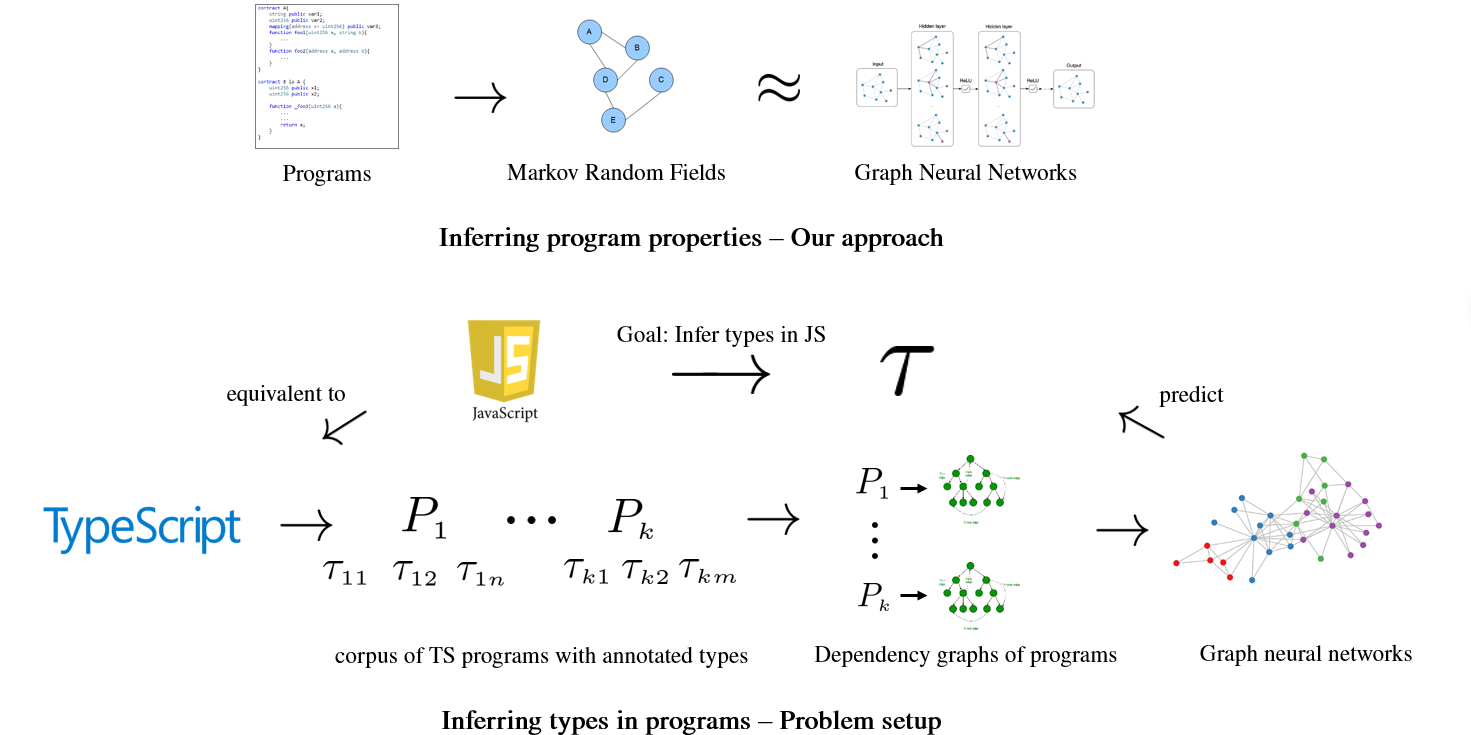
\includegraphics[width=\textwidth]{img/architecture.png}
	}
	\caption{\textbf{Summary of our work.} We motivate the problem of modeling programs as Markov Random Fields. We argue that a graph neural network approximates inference over a MRF. Specifically, we investigate the problem of inferring types in JavaScript programs. This problem formulation was first put forward by Allamanis \textit{et al.}~\cite{hellendoorn2018deep}.}
	\label{fig:pipeline}
\end{figure*}
%</figPipeline>

%<*baseline>
\begin{figure}
	\centering
	\scalebox{0.7}{
		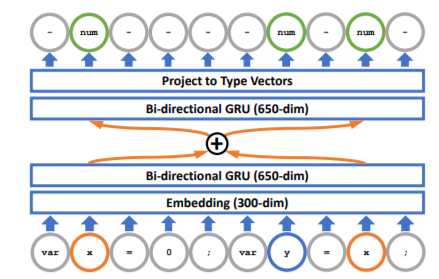
\includegraphics[width=\linewidth]{img/birnn.png}
	}
	\caption{Aggressive baseline - A bi-directional RNN designed by Allamanis \textit{et al.}~\cite{hellendoorn2018deep}. It models type inference as a sequence prediction task in NLP.}
	\label{fig:birnn}
\end{figure}
%</baseline>

%<*gnn>
\begin{figure}
	\centering
	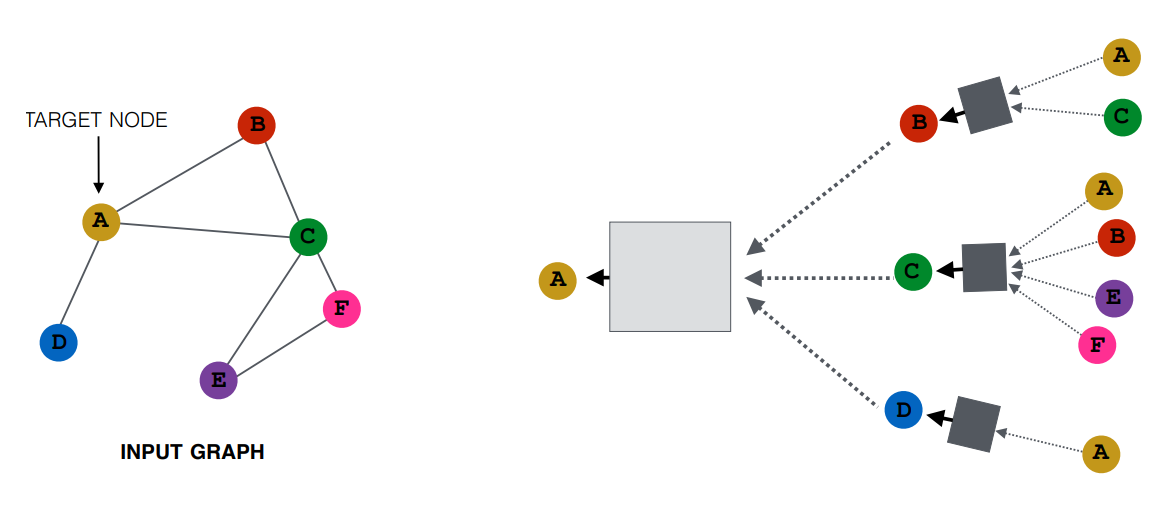
\includegraphics[width=\linewidth]{img/gnn.png}
	\caption{A typical graph neural network architecture, from~\cite{leskovec2018representation}. The key idea is to generate node embeddings based on neighborhood information.}
	\label{fig:gnn}
\end{figure}
%</gnn>

%<*labelDistribution>
\begin{figure}
  \centering
  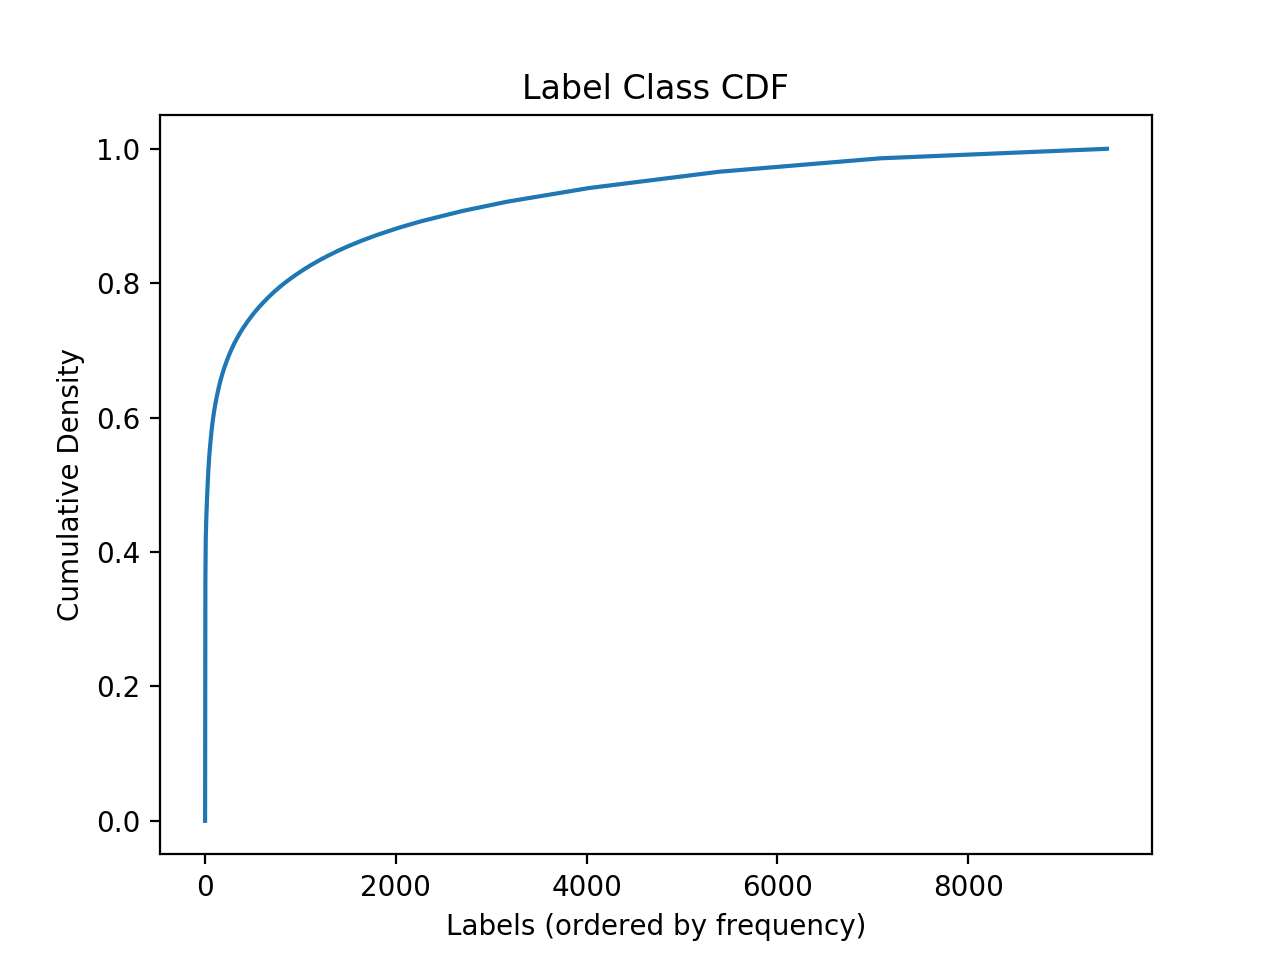
\includegraphics[width=0.7\linewidth]{img/label_cdf}
  \caption{CDF of label frequencies in the dataset.}
  \label{fig:label-distribution}
\end{figure}
%</labelDistribution>

%<*astDistribution>
\begin{figure}
  \centering
  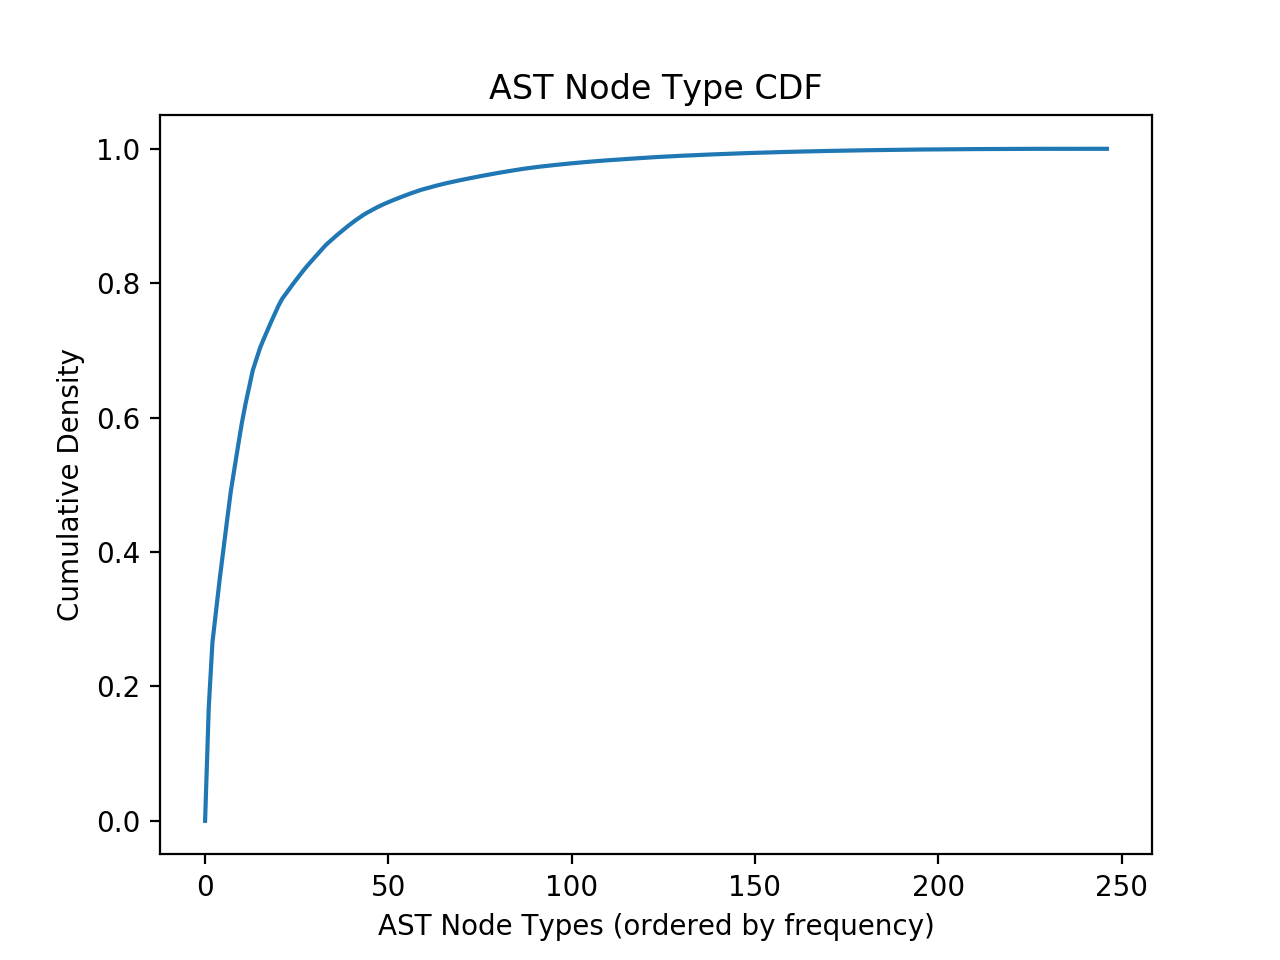
\includegraphics[width=0.7\linewidth]{img/ast_cdf}
  \caption{CDF of AST type frequencies in the dataset.}
  \label{fig:ast-distribution}
\end{figure}
%</astDistribution>

%<*stats>
\begin{figure}
	\centering
	\begin{subfigure}{0.49\linewidth}
		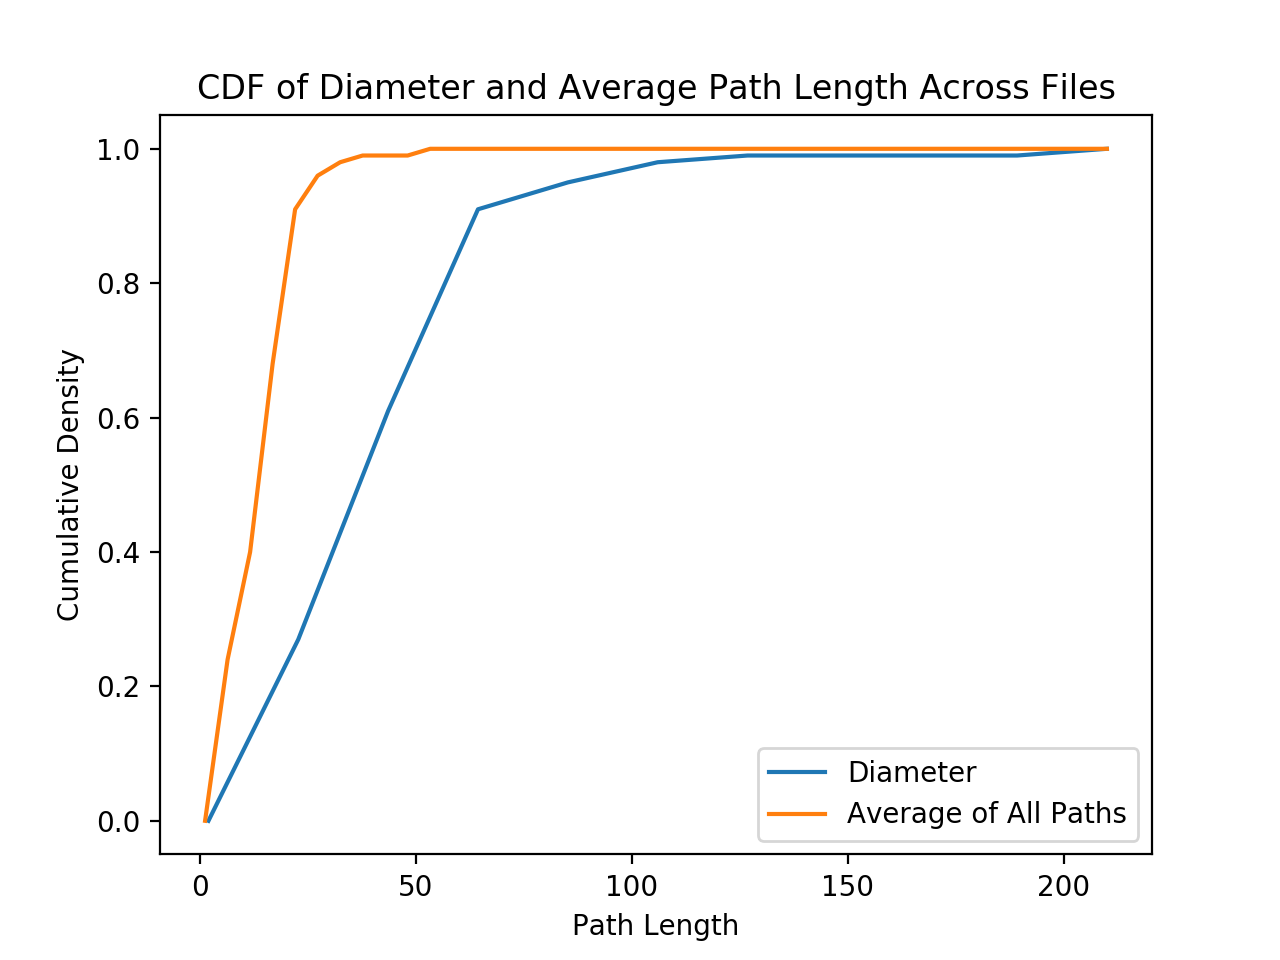
\includegraphics[width=\textwidth]{img/diameter}
		\label{fig:g1}
	\end{subfigure}
	\begin{subfigure}{0.49\linewidth}
		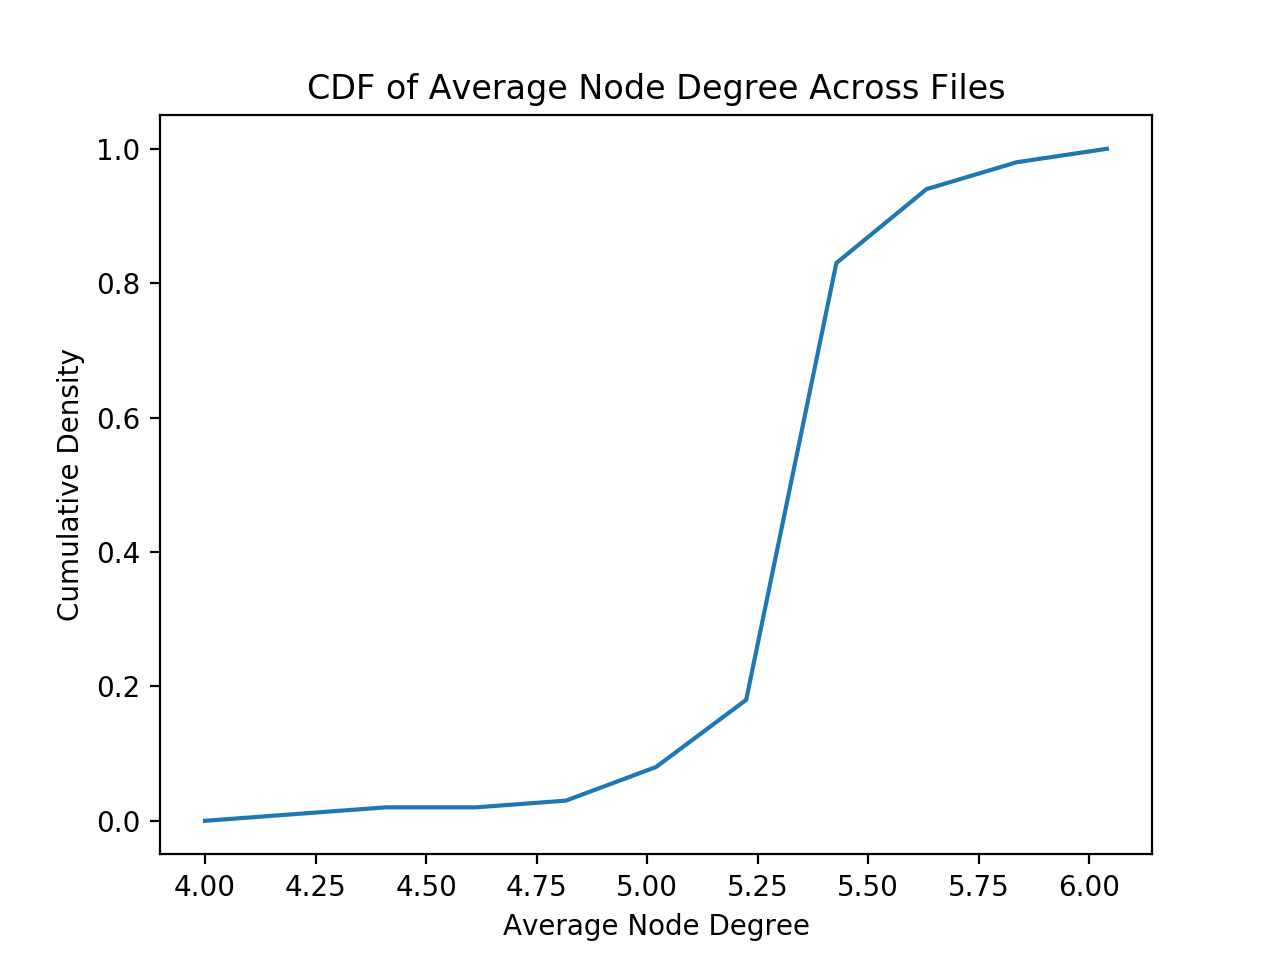
\includegraphics[width=\textwidth]{img/node_degree}
		\label{fig:g2}
	\end{subfigure}
	\caption{A summary of key dataset statistics, showing the CDFs of the average path length, and the average node degrees of the graphs in the dataset. }
	\label{fig:dataset-graph-stats}
\end{figure}
%</stats>

%<*gpDiagram>
\begin{figure}
	\centering
	\scalebox{0.9}{
	    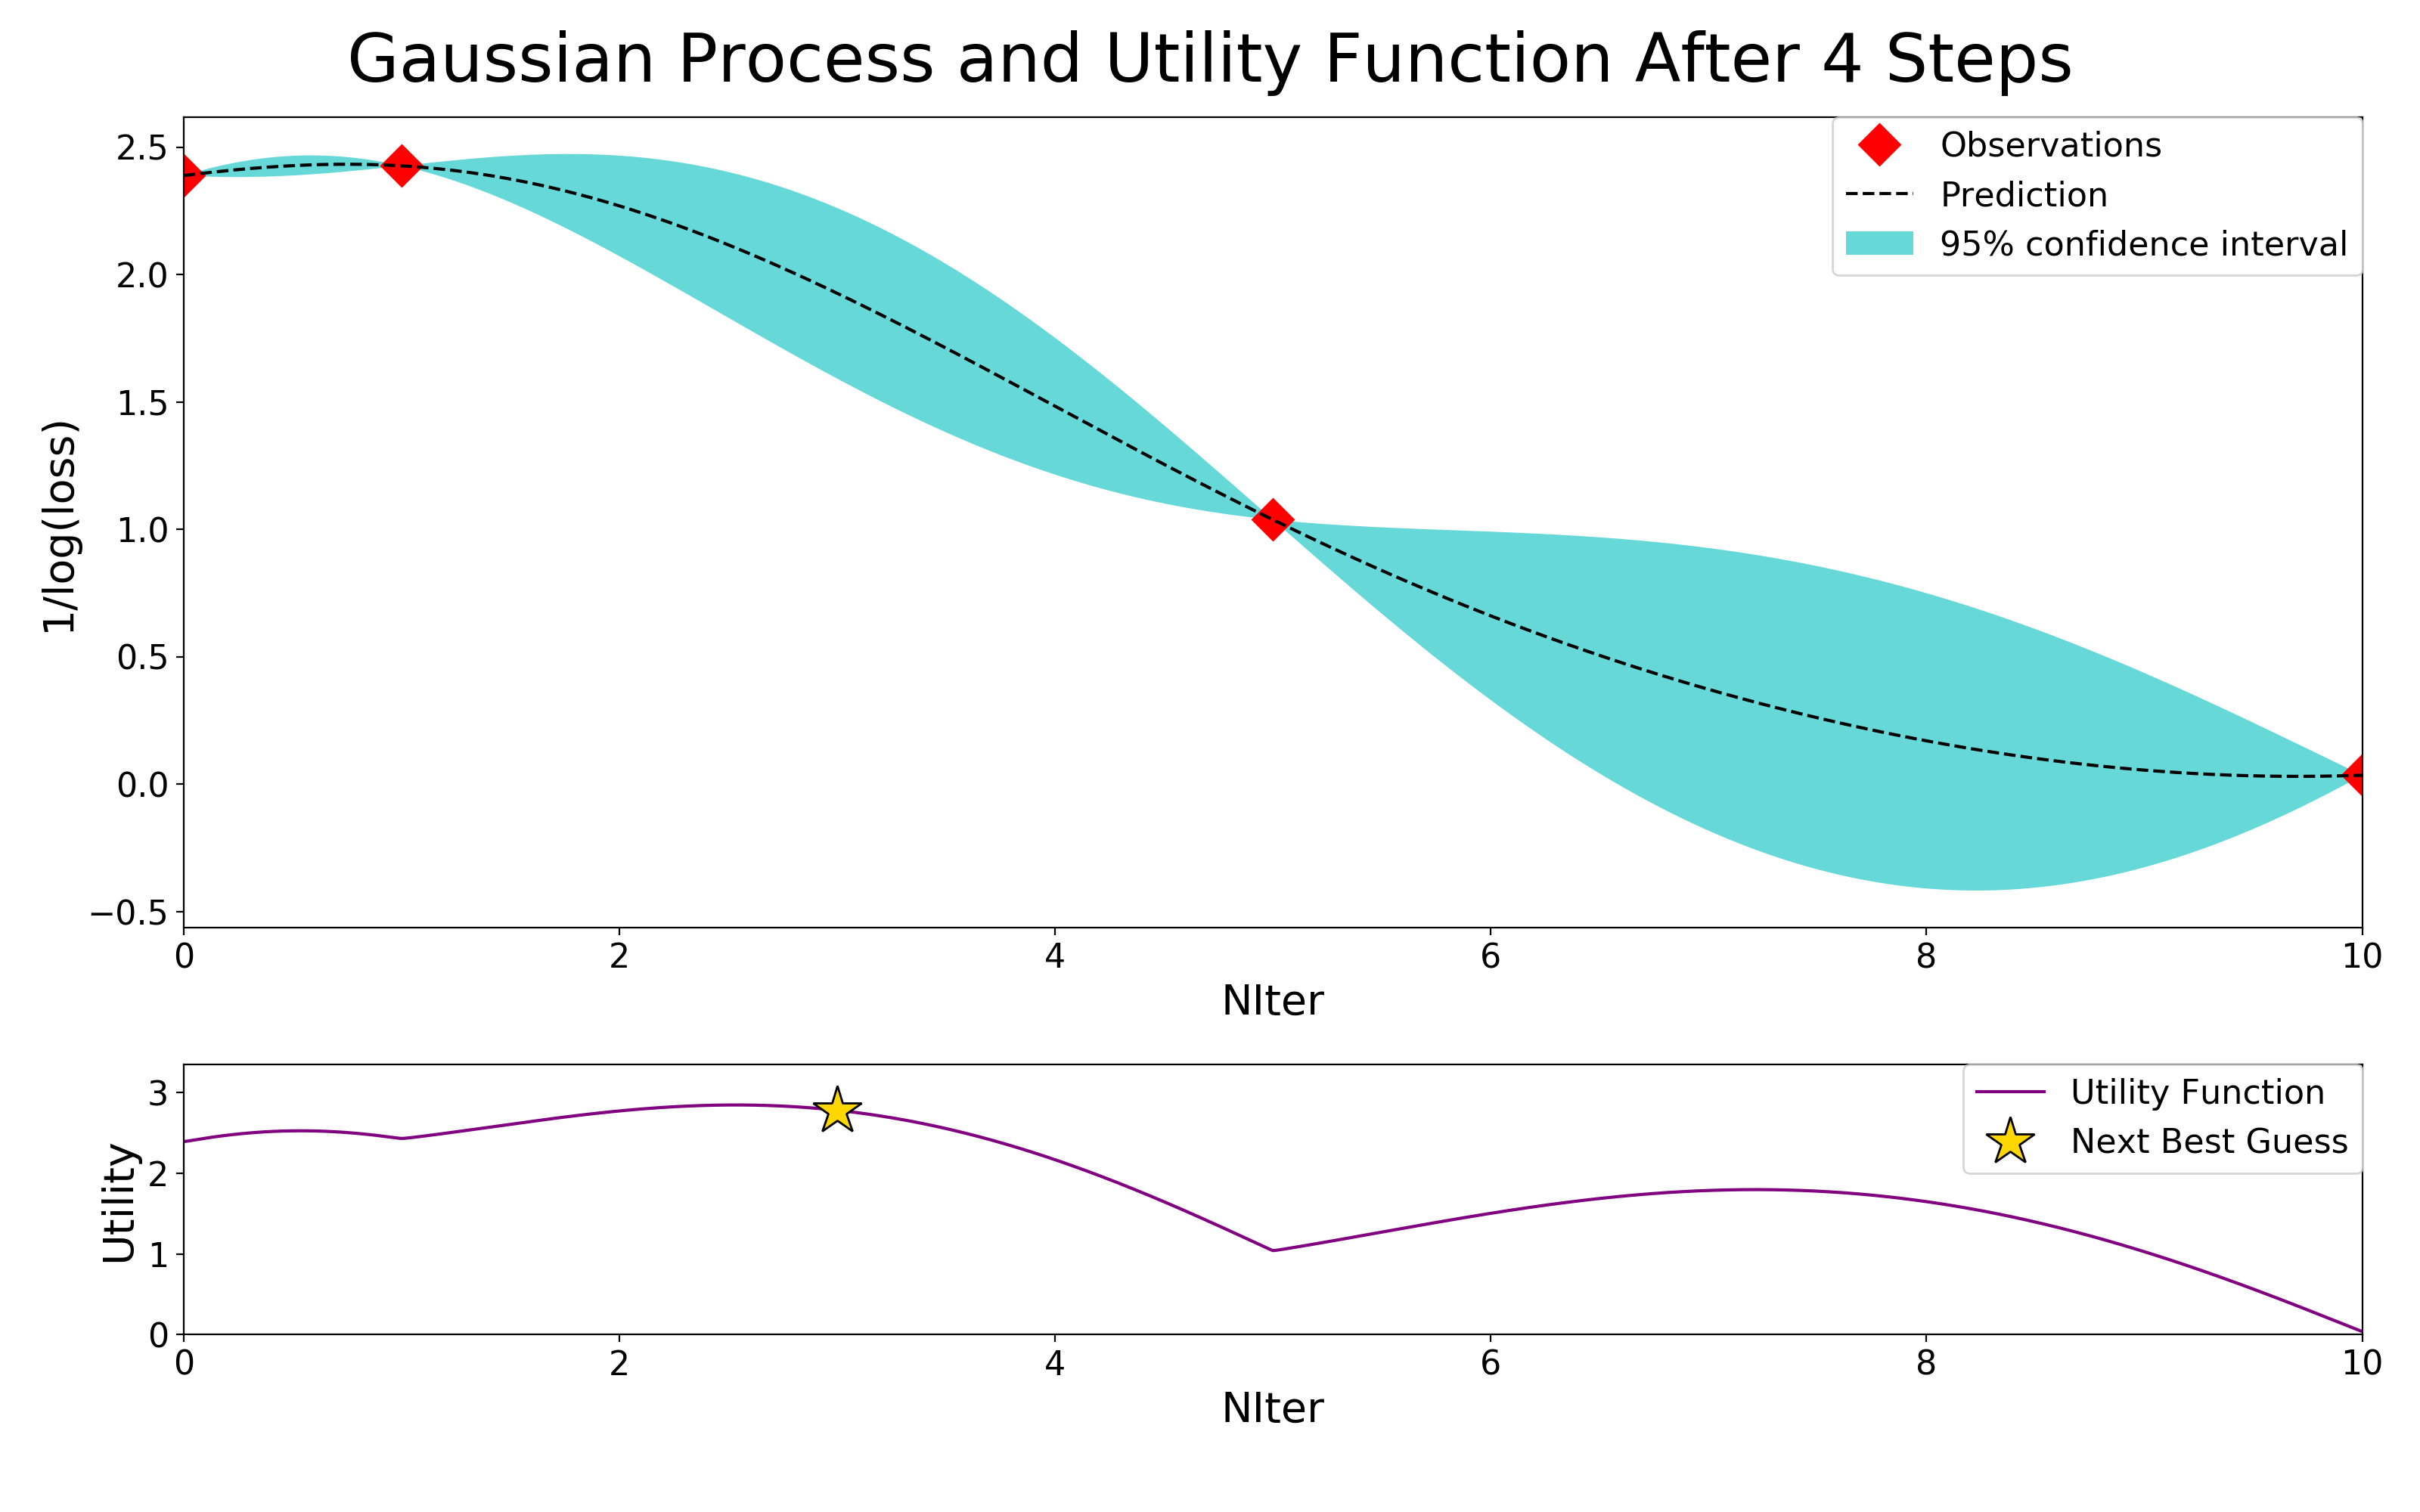
\includegraphics[width=\linewidth]{img/bo}
	}
	\caption{Partial result of Bayesian Optimization on \textsc{NIter} (after 4 samples)}
	\label{fig:gp-diagram}
\end{figure}
%</gpDiagram>

%<*graph>
\begin{figure}
	\centering
	\scalebox{0.8}{
		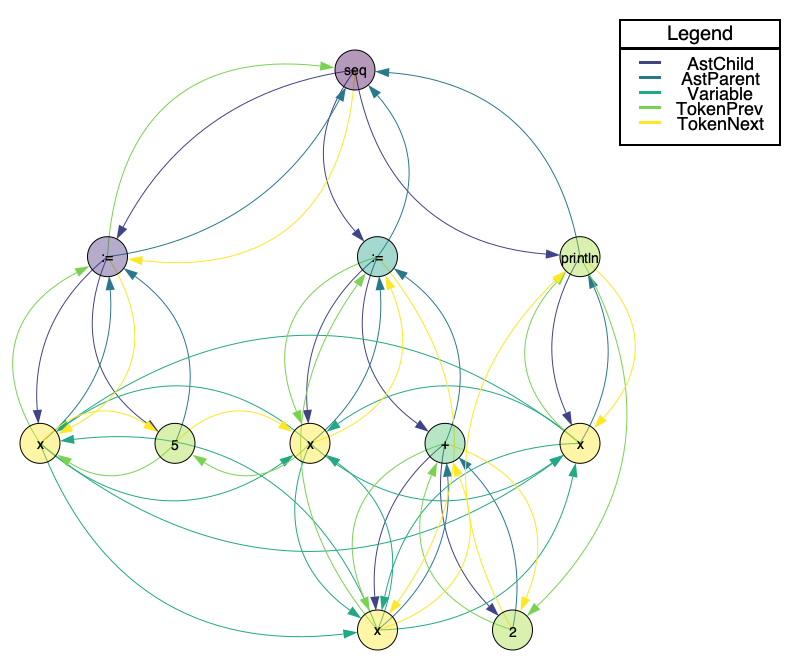
\includegraphics[width=\linewidth]{img/gen_graph}
	}
	\caption{Generated graph for a simple example}
	\label{fig:ast-graph}
\end{figure}
%</graph>

%<*mrf>
\begin{figure}
	\centering
	\scalebox{0.7}{
		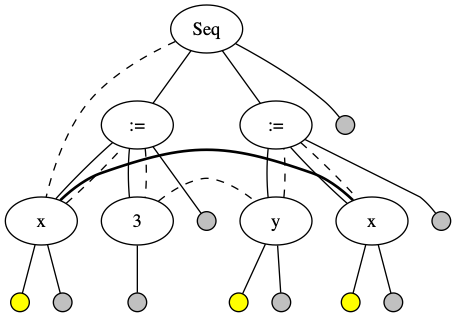
\includegraphics[width=\linewidth]{img/mrf_graph}
	}
	\caption{Constructed Markov Random Field for an example program: \mbox{\texttt{x := 3; y := x;}} Shaded nodes are observed, highlighted are desired posteriors}
	\label{fig:mrf-graph}
\end{figure}
%</mrf>
